Para se ter uma noção da disposição de casos de COVID-19 em Manaus, foi feito um estudo sobre a distribuição percentual de ocorrências, levando em consideração um agrupamento por bairros. Tendo isso em vista chegou-se ao seguinte gráfico da Figura~\ref{fig:uc3} que demonstra os 10 bairros com maior percentual de afetados (eixo x) e seus respectivos percentuais (eixo y), todos os demais bairros encontram-se juntos agrupados pelo rótulo de 'OUTROS'. Observa-se que existe certa uniformidade entre os bairros com maior índice de contaminados.
\begin{figure}[!ht]
\centering
    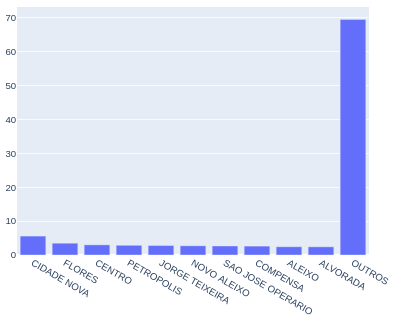
\includegraphics[width=6.8cm]{img/percentualPorBairro.png}
    \caption{Gráfico de percentual nos 10 bairros de maior ocorrência}
    \label{fig:uc3} % Toda figura tem que ter um label diferente
\end{figure}

Em adição a isso percebe-se que a variação entre os dados é de certa forma bem significante, para exemplificar isso foi feito o boxplot de casos confirmados por idade que estão mostrados na Figura~\ref{fig:uc4} e é perceptível a presença de \textit{outliers} (valores discrepantes) de forma expressiva na faixa 82 a 100 anos. Em conjunto com a Figura~\ref{fig:normal}, nota-se que as caudas da distribuição são largas e a dispersão  é baixa visto pelo tamanho da caixa representando os quartis. Os \textit{outliers} mostram que mesmo os mais idosos, acima de 100 anos e que são minoria, e as crianças mais novas, não foram privados do contágio, visto que de acordo com a Figura~\ref{fig:normal}, existe um pico para os recém nascidos.

\begin{figure}[!ht]
\centering
    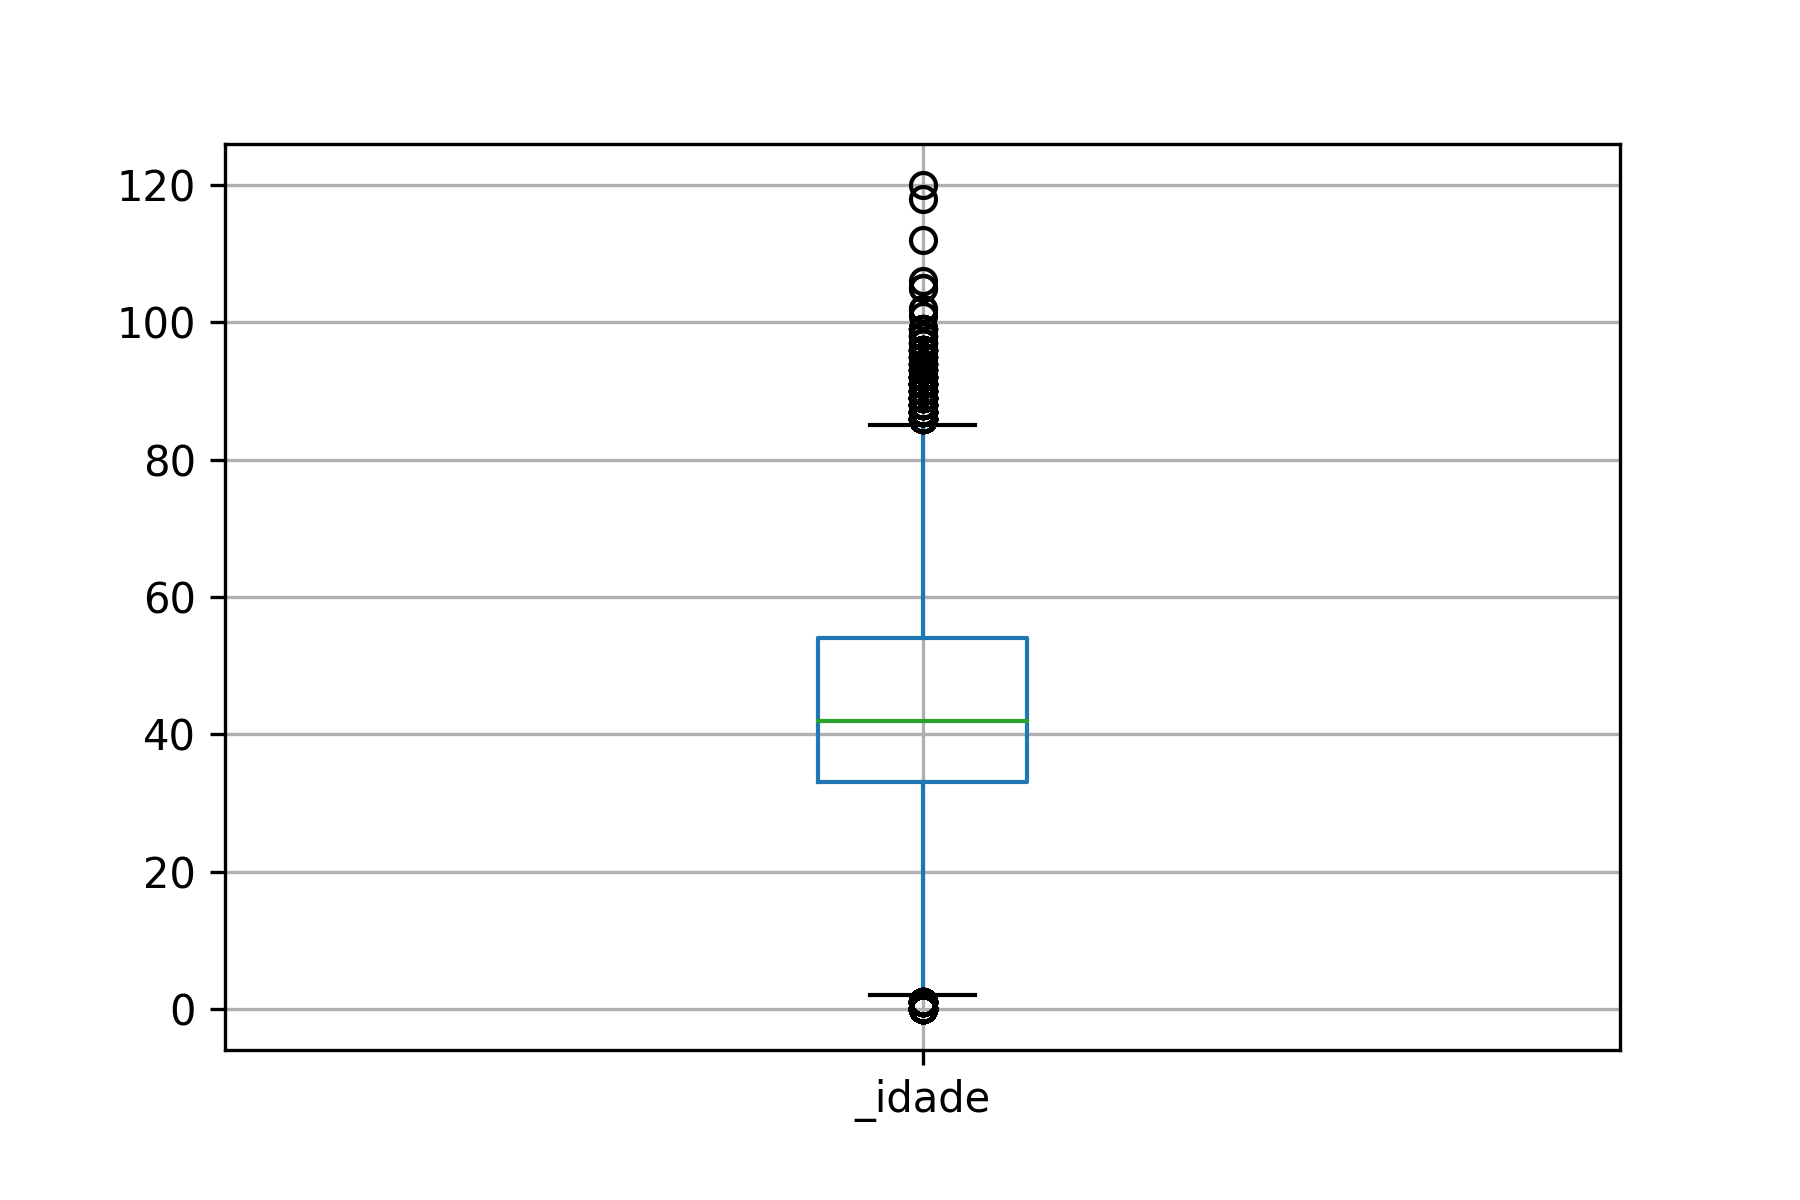
\includegraphics[width=8cm]{img/boxplot.png}
    \caption{Boxplot da idade dosS casos confirmados}
    \label{fig:uc4} % Toda figura tem que ter um label diferente
\end{figure}

Com um intuito de sensibilização do nível de contaminação do vírus, foi feito um gráfico, figura~\ref{fig:uc5}, que mostra a quantidade de novos casos confirmados nos últimos 10 dias contidos na base de dados, e também, para critério comparativo, foi feito um segundo gráfico similar ao da figura~\ref{fig:uc5} mas, levando em consideração a quantidade de pessoas recuperadas. O mesmo é representado pela figura~\ref{fig:uc6}. 

Como é possível constatar, a ocorrência de novos casos é muito mais recorrente que a de casos recuperados. Isso demonstra que a incidência do vírus tende a aumentar cada vez mais. É possível perceber também que todos os dias ouve novas notificações de casos enquanto de recuperados não.
\begin{figure}[!ht]
\centering
    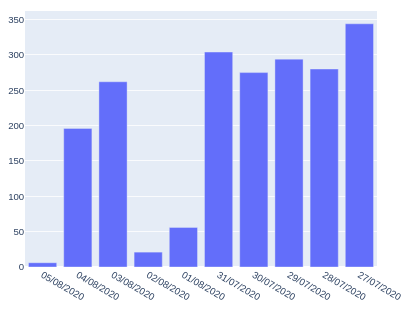
\includegraphics[width=8cm]{img/ultimos10dias.png}
    \caption{Número de novos casos por dia, considerando os 10 últimos dias existentes na base de dados}
    \label{fig:uc5} % Toda figura tem que ter um label diferente
\end{figure}
\begin{figure}[!ht]
\centering
    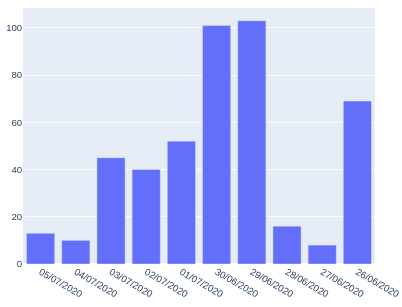
\includegraphics[width=8cm]{img/ultimos10diasConfirmados.png}
    \caption{Número de novos casos recuperados, considerando os 10 últimos dias existentes na base de dados}
    \label{fig:uc6} % Toda figura tem que ter um label diferente
\end{figure}

Visando analisar a quantidade de casos do vírus em relação as idades, foi feito um histograma, apresentado na figura 9, no qual é apresentado a relação Porcentagem x Faixa etária. Pelo histograma (figura 9), notamos que a quantidade de casos é baixa para as faixas etárias mais jovem e vai crescendo até 31 a 40 e 41 a 51. Depois disso, começa a cair, gerando assim, uma figura muito parecida com uma distribuição normal. Isso mostra que pessoas com idade de trabalho, provavelmente as que tiveram que sair de suas casas, ficaram mais vulneráveis ao vírus.

\begin{figure}[!ht]
\centering
    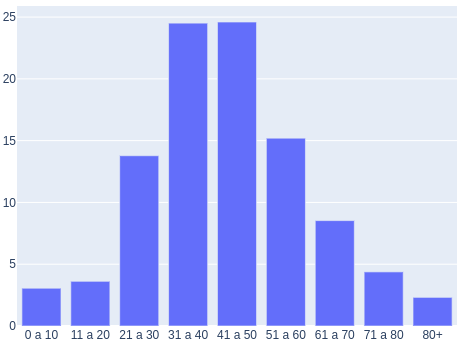
\includegraphics[width=8cm]{img/procentagemporidade.png}
    \caption{Histograma Porcentagem de Casos x Faixa etária}
    \label{fig:uc7} % Toda figura tem que ter um label diferente
\end{figure}

Para efeito demonstrativo o gráfico da figura~\ref{fig:uc8} mostra a curva da quantidade total de casos ao longo do tempo. Ao observar esse gráfico facilmente nota-se que a curva é ascendente com uma inclinação bem acentuada mas que por volta do mês 06 sofreu um pequeno desvio e seus valores começaram a diminuir (ainda sim é muito inclinada) semelhante a uma função logarítmica mas que ainda não chegou em seu ponto de equilíbrio e que mostra um possível aumento ainda nos meses seguintes.
\begin{figure}[!ht]
\centering
    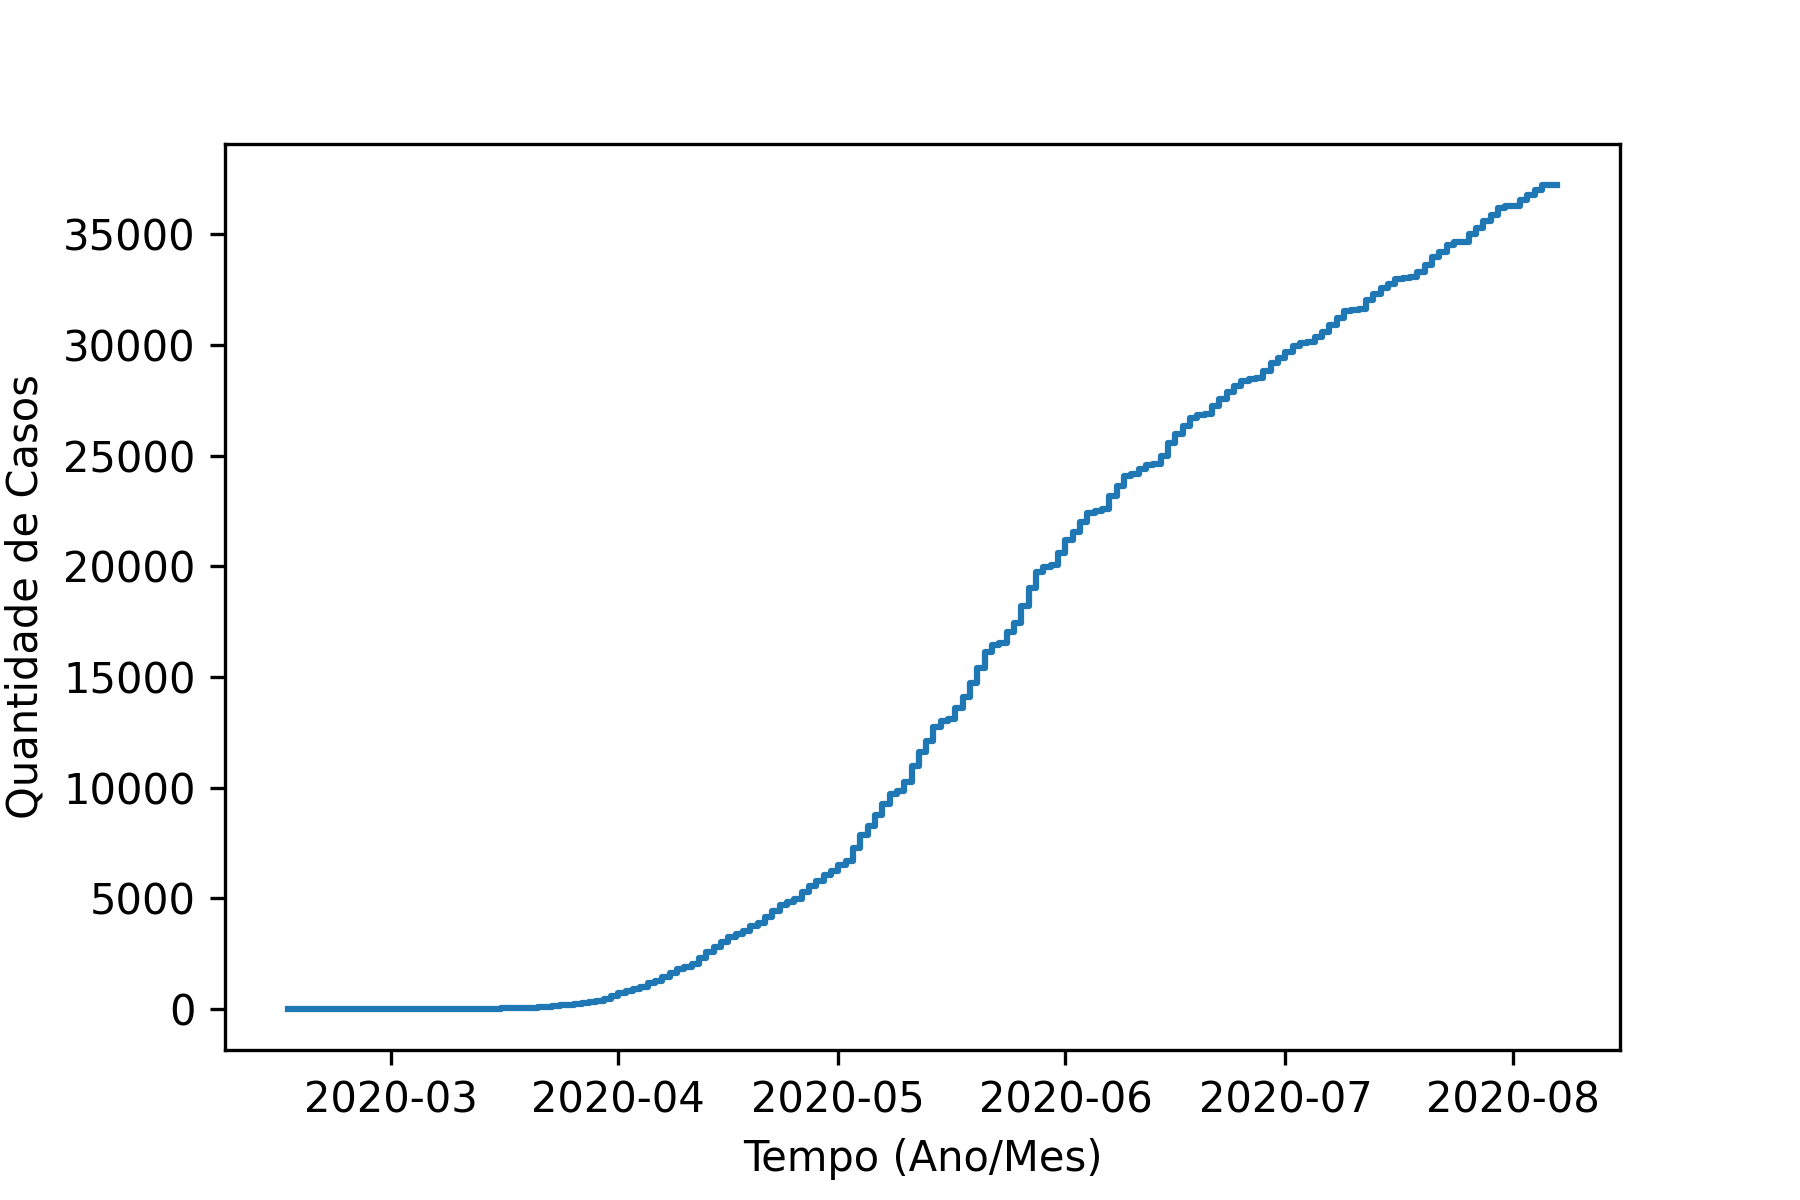
\includegraphics[width=9cm]{img/distribuicao2.6.png}
    \caption{Gráfico cumulativo de casos notificados ao longo do tempo}
    \label{fig:uc8} % Toda figura tem que ter um label diferente
\end{figure}

Já no gráfico~\ref{fig:uc9}, podemos ver um gráfico que denota a idade relacionada ao total de casos registrados para aquela certa idade, ou seja, usando os dados brutos. Comparando ao gráfico~\ref{fig:normal}, os dois são muito semelhantes, em ambos os gráficos, existe a tendência que os mais afetados são aqueles com aproximadamente 40 anos, mas também houve um pequeno pico nos recém-nascidos. Ou seja, o trabalhador médio que é em sua maioria na faixa de 40 anos estava mais sujeito a contaminação, nos extremos, a intensidade é menor porém ela é uniformemente distribuída e os recém nascidos foram bastante vulneráveis. 
\begin{figure}[!ht]
\centering
    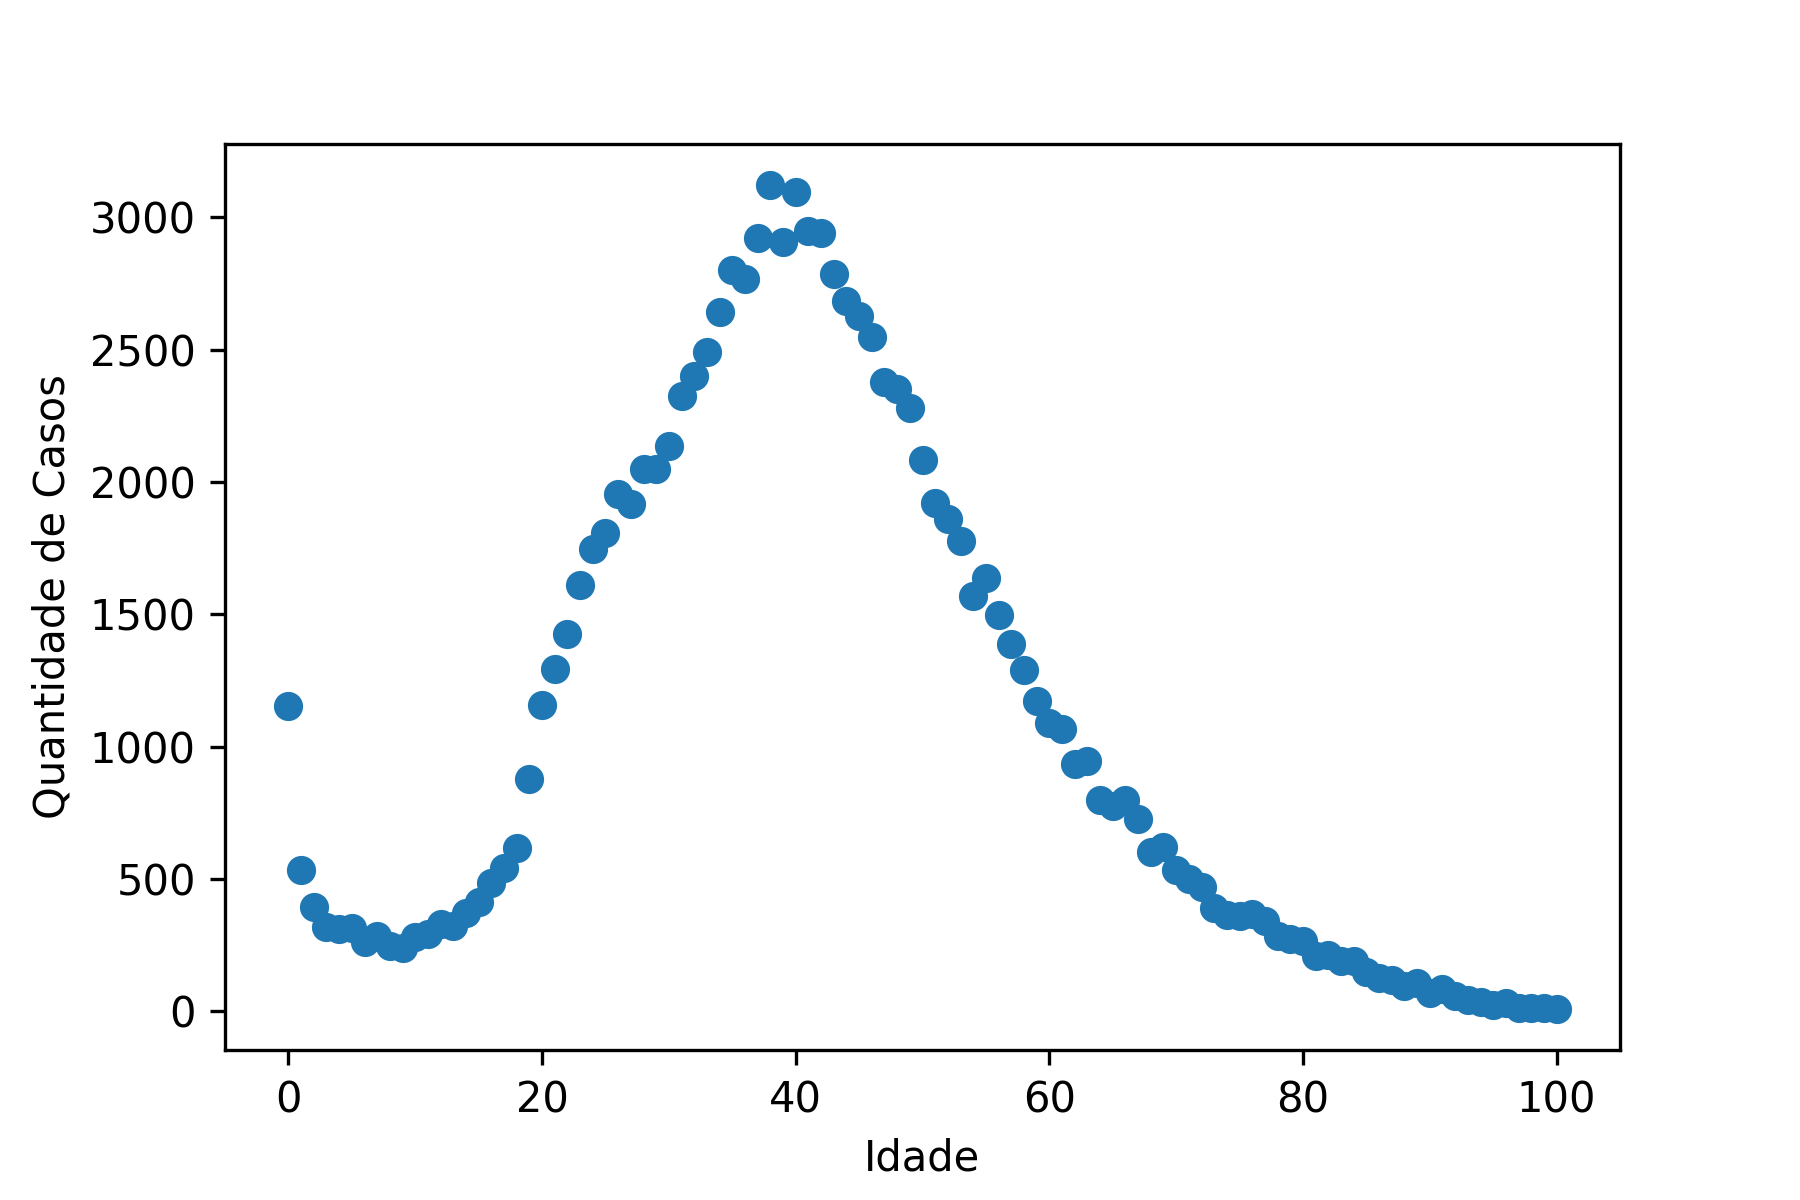
\includegraphics[width=9cm]{img/distribuicaoPorIdade2.7.png}
    \caption{Gráfico da idade versus o número total de casos registrados. Todos os casos registrados}
    \label{fig:uc9} % Toda figura tem que ter um label diferente
\end{figure}